\documentclass[titlepage]{article}
\usepackage{listings}
\usepackage{graphicx}
\graphicspath{ {images/} }
%\usepackage[numbers, square, sort]{natbib}
\usepackage[left=1in, top=1in, right=1in, bottom=1in, nohead]{geometry}
\title{Comparing Algorithms for the Sparse Group Lasso}
\author{Aaron Cohen}
\begin{document}
    \maketitle
    \begin{abstract}
        In this paper we explore two algorithms for the sparse group lasso. 
    \end{abstract}

\section{1. Introduction}
The lasso is "a regression analysis method that performs both variable selection and regularization" which uses an $l1$ penalty to select a subset of predictors to be nonzero. It is of the form 
\[
min_{\beta} ||y-X\beta||_2^2 + \lambda ||\beta||_1
\]
A variant of this, the group lasso is appropriate when there is a naturally grouped structure for the predictors $\beta = (\beta^{(1)},\ \beta^{(2)},\ \dots, \ \beta^{(m)})$; it performs regularization that has the effect of selecting for the groups of predictors rather than the predictors themselves. It is of the form 
\[
min_{\beta}\frac{1}{2}||y-\sum_{l=1}^mX^{(l)}\beta^{(l)}||_2^2 + \lambda\sum_{l=1}^m\sqrt{p_l}||\beta^{(l)}||_2
\]
Finally, in a grouped-structure problem as above it may be desirable to enforce sparsity not only among the groups but within the groups, as well. The sparse group lasso solves this with the following minimization problem
\[
min_{\beta}\frac{1}{2}||y-\sum_{l=1}^mX^{(l)}\beta^{(l)}||_2^2 + (1-\alpha)\lambda\sum_{l=1}^m\sqrt{p_l}||\beta^{(l)}||_2+\alpha\lambda||\beta||_1
\]
Note the tuning parameter $\alpha$ which controls the relative emphasis of intra- vs inter- sparsity in the predictors.

In this paper we consider solving the sparse group lasso for a whole range of parameters $(\lambda_1,\dots \lambda_n)$ rather than a single value, and a computational problem presents itself:  can we speed up the algorithm at a  given $\lambda_i$ by utilizing the solution at the previous $\lambda_{(i-1)}$? A heuristic solution to this, used in the present paper, is the Strong Rule, which predicts which predictor (groups) will remain zero at the solution for $\lambda_i$ and throws them out. If a significant number of groups are thrown out before entering the algorithm, convergence time can iprove significantly.

There are already two other existing R packages that perform group lasso, gglasso and sgl. The advantage of our package over those two are as follows: the sgl package has sparsity, but does direct coordinate descent and does not have a heuristic like the strong rule, so it does not take advantage of such a computational speedup. The gglasso package, on the other hand, incorporates such a rule and is computationally fast, but does not incorporate within-group sparsity. Our contribution, then, is to provide a package that performs sparse group lasso, and is faster than existing algorithms. This algorithms for this package are written in Fortran, and are based on the algorithm from the gglasso package.

In section 2, we describe the algorithm in detail, paying particular attention to the strong rule. In section 3, we show how to use the package, running through an example with simulated data. In section 4, we compare our package to the other existing sgl package, and also compare the two variants of our algorithm with each other.

\section{Methodology}

\subsection{Overview of the algorithm}

There is no closed-form solution to the optimization problem above, so we need a numerical algorithm to find the optimal solution. The general framework for both of our algorithms is based on (groupwise) coordinate descent. That is, we loop over the groups and, for a given group, update only those variables while holding all other groups constant. First, we note that the loss $l$, being quadratic, can be dominated by the following:

\[
\forall \beta,\beta^*,\ \ell(\beta) \leq \ell(\beta^*)+(\beta - \beta^*)^T\nabla \ell(\beta^*)+\frac{1}{2}(\beta - \beta^*)^T H (\beta - \beta^*)
\]

where $H = tI$ and $t$ is the largest eigenvalue of the Hessian. This reduces computation significantly, as the $t$ factors out and removes the need for matrix multiplication.

We take the original minimization equation and replace the loss with the above. This can be solved, with the resulting update step that $\beta^{(k)}$ is replaced by

\[
\left(1-\frac{t(1-\alpha)\lambda}{||S(\beta^{(k)}-t\nabla \ell(r_{-k)},\beta^{(k)}),\ t\alpha\lambda)||_2}\right)_+ S(\beta^{(k)}-t\nabla \ell(r_{(-k)},\beta^{(k)}),t\alpha\lambda)
\]

where  $S$ is the coordinate-wise soft-threshold operator $(S(a,b))_j = sign(a_j)(|a_j|-b)_+$. Note that in updating $\beta^{(k)}$ it is possible for the whole group to be set to zero (made inactive) because of the threshold operator $()_+$ in the first part of the expression, and/or for individual components of $\beta^{(k)}$ to be zeroed out from the coordinate-wise threshold $S()$. So this algorithm setup performs variable selection at both the group and individual level.

Because the optimization problem is convex, it can be shown that this type of descent algorithm is guaranteed to converge to the optimal solution. That is, it does not get 'stuck' at any inflection points. Therefore, if that was all the algorithm did, there would be no need to check the KKT conditions for optimality. 

However, our algorithms both make use of a heuristic that predicts, before computation, which groups will remain inactive, and throws them all out; this results in significant computational savings, but because of this pre-processing prediction, we will need to do a KKT check to make sure the prediction was accurate. This is described in the next section.

\subsection{Strong Rule}

As mentioned above, the strong rule is a heuristic that is easy and fast to perform, throwing away large numbers of predictors before computation, but it is not guaranteed to be correct, so it becomes necessary to double-check the solution with the KKT check afterwards. 

It is important to note first of all that the version of the strong rule used here, the sequential strong rule, makes critical use of the fact that we are solving for a sequence of $\lambda$ parameters---without loss of generality assume that the problem has already been solved for the previous $\lambda_{k-1}$.

The motivation for the strong rule comes from the KKT check, so we start with this.

The KKT stationarity condition for this problem is 

\[
||S(X^{(k)T}r_{(-k)}/n,\ \alpha\lambda)||_2 \leq (1-\alpha)\lambda
\]
The left-hand side of this inequality is the norm of the (sub)gradient of the loss $l = l(r_{(-k)},\beta)$, where $r_{(-k)}= y - \sum_{\ell \neq k} X^{(l)}\beta^{(l)}$.

Denote 

\[
c_j = c_j(\lambda) = S(X^{(j)T}r_{(-j)}/n,\ \alpha\lambda),
\]
i.e., $c_j$ at a given $\lambda$ in the sequence is the subgradient with respect to the $j$-th group.

The (sequential) strong rule checks if the following inequality holds, and discards the $j$-th group if so:

\[
|c_j(\lambda_{k-1})| < (1-\alpha)(2\lambda_k - \lambda_{k-1})
\]

The reasoning is as follows: consider $c_j(\lambda)$ as a function of lambda. The key point is that, if this function $c_j$ were $(1-\alpha)$-Lipschitz, by definition it would satisfy
\[
|c_j(\lambda) - c_j(\tilde{\lambda})|\leq (1-\alpha)|\lambda-\tilde{\lambda}|
\]
Now suppose it were Lipschitz and also that $c_j(\lambda_{(k-1)}$ were known, i.e. we have solved the problem for the previous lambda in the sequence. Then, \underline{when the strong rule is satisfied}, we combine the two previous inequalities to get
\[
|c_j(\lambda_k)|\leq (1-\alpha)(|c_j(\lambda_k) - c_j(\lambda_{k-1})|+|c_j(\lambda_{k-1})|)<(1-\alpha)(\lambda_{k-1}-\lambda_k+2\lambda_{k}-\lambda_{k-1})
\]
which is precisely the KKT stationarity condition at $\lambda_k$. Thus, if the strong rule condition were satisfied at this group (and assuming the Lipschitz condition, which is not always true), it follows that $\beta_j$ is inactive for the current lambda, $\lambda_k$. Since we made the Lipschitz assumption, which essentially says that $c_j$ does not change "too fast" as a function of $\lambda$, we need to check after performing the algorithm on the other groups that this group is indeed inactive. In fact, as shown in the strong rules paper (), it is very often the case that the $c_j$'s are $(1-\alpha)$-Lipschitz.

\subsection{The three-step and four-step algorithm}

There are two algorithms in our package that perform sparse group lasso: the three-step algorithm and the four-step algorithm. First we discuss the three-step.

In the initialization (step 0) of the algorithm, we set the lambda path (the decreasing set of $\lambda$ 's which comprise the parameter space), and start keeping track of two sets, $\mathcal{E} = \emptyset = \mathcal{A}$ , which are initially empty. Both of these sets grow as the algorithm is run; predictors get put into these groups if they pass certain checks, but never leave once they are put in.

Without loss of generality assume that we have run the algorithm for a few lambdas, and are at $\lambda = \lambda_{k}$. The first step (step 1) of the algorithm is to run the strong rule check on all predictor groups in $\mathcal{E}^c$, and every group that passes the strong rule (which is computed using the gradient at the previous lambda) gets put in the set $\mathcal{E}$. So $\mathcal{E}$ is essentially keeping track of every predictor that has ever passed the strong rule check--these are candidates for active groups.

In the second step (step 2), we loop over $\mathcal{E}$, performing the update step until convergence. Again, this is a type of coordinate descent, but we are saving a lot of time by keeping all groups in $\mathcal{E}^c$ zero and only updating on those suspected of being active. Now, although $\mathcal{E}$ is keeping track of the 'strong set', any time a group actually becomes active (i.e. is updated to be nonzero), it gets put in $\mathcal{A}$, the 'active' set. This is because while we save the indices of the potentially-active groups, we only save the values of the actually active groups.

Finally, after we have converged (the update step for all groups is changing values by less than a small epsilon), we need to perform the KKT check to make sure that we didn't accidentally leave some active groups at 0. Again, if we were not using the strong rule check, this would be unneccessary. The only potential violators are in the complement of $\mathcal{E}$, so: run the KKT check on $\mathcal{E}^c$, throw any violators into $\mathcal{E}$ and go back to step 2. If there are no violators, we have found the solution at the given $\lambda$, so we save the values in $\mathcal{A}$, as well as the gradients, and move on to the next lambda.

The four-step algorithm has a slight refinement over the three-step. It is as follows. First note that there is only one set to keep track of, the set $\mathcal{E}$. The setup is the same.

Assume we have solved the problem for $\lambda_{k-1}$. We loop over $\mathcal{E}$ and update until convergence. The difference here is that we do not perform the strong check first. After we have run the update loop until convergence on our set, we then perform the strong rule on the complement, $\mathcal{E}^c$. For any groups that pass the strong rule, we run the kkt check; if there are any violators, put them in $\mathcal{E}$ and go back to step 1. 

Otherwise, we run the full KKT check, the KKT check on the full complement $\mathcal{E}^c$. Again, if there are any violators, we put them in $\mathcal{E}$ and go back to step 1. If there are no violators, we are done, and we move on to the next $\lambda$ in the sequence.



\section{Example}

In this section we provide a worked-through example of how the package is used. 

First, we generate some random data. There will be $n=100$ observations and $p=200$ predictors. The predictors will be partitioned into groups of 5, so e.g. the first five predictors form the first group, and so on. Some of the groups will be inactive ($0$), and within a given active group, some of the variables will be $0$. The goal is to learn exactly this information.

Once we make a random design matrix $X$ and the true $\beta$ vector (which has the group structure mentioned above), we form the response vector $y$ according to $y=X\beta + \epsilon$. The following code generates the data for this example.

\begin{lstlisting}[language=R]
set.seed(1010)
n <- 100
p <- 200
X <- matrix(data = rnorm(n*p, mean=0, sd=1), nrow = n, ncol = p)
eps <- rnorm(n, mean = 0, sd=1)
beta_star <- c(rep(5,5), c(5,-5,2,0,0), rep(-5,5), c(2,-3,8,0,0), rep(0,(p-20)))
y <- X%*%beta_star + eps
groups <- rep(1:(p/5), each=5)
\end{lstlisting}

Since we generated the data according to the above equation, we know the true value of $\beta$, in particular which groups are active and which predictors within active groups are nonzero. We want to use the sparsegl package to backsolve: given $X,\ y$ and the group partition information (how the predictors are divided up into groups, but not the values), how can we best estimate the predictors $\beta$?

To reiterate, we need to know beforehand how the predictors are divided up into groups; the algorithm takes that in, and does not learn it. Also note that the groups in $\beta$ are contiguous. The data needs to be grouped in such a way before we can apply our package.

This package will estimate $\beta$ for a whole path of $\lambda$ weights. For each $\lambda$, it will find the optimal solution for that weight, according to equation <blank>. The lambda path can be explicitly specified as an input, but otherwise it creates its own set of $\lambda$, first finding the smallest value of $\lambda$ that forces all predictors to be zero, and decrementing logarithmically 100 times, to get a set of 100 decreasing $\lambda$'s. For this particular dataset, the lambdas range from $0.636$ to $0.00636$, with log-constant decremental step-size.

In addition to lambda we also need to set $\alpha$, which controls the relative emphasis on inter- vs intra- group sparsity. The default is $\alpha = 0.05$. Here is the code that runs the algorithm and stores the results in an object called mysparse1.

\begin{lstlisting}[language=R]
mysparse1 <- sparsegl(x = X, y = y, group = groups,
                         pen = "sparsegl", algorithm = "threestep")
\end{lstlisting}
With the above line of code, we have run the algorithm that solves the problem for the default lambda space, and created a sparsegl object. The main data in that object is the $B$ matrix, which gives the estimated beta vector for each value of $\lambda$. Note that, when calling this function, we must give it the group structure, and also specify the threestep vs the fourstep algorithm. Finally, the 'pen' flag specifies that we want to perform sparse group lasso; there is also the option to just perform group lasso.

If we look now at the $B$ matrix, we see that, for a particular range of lambdas, the algorithm was able to deduce correctly the active groups, the active predictors within those groups, and accurately estimate their weights.

<<see beta matrix>>

It is illustrative to look at a graph of the predictors against lambda, to see when the various predictors become active. For visualization reasons, we instead plot on the x-axis, not lambda but an equivalent measure, the relative group norm. This is equivalent to graphing against lambda, since as lambda \underline{decreases}, the group-norm (which is the sum of $L_2$ norms of all the groups in beta) of the fitted beta increases. This type of graph is produced by a built-in function of the sparsegl package. All predictors are plotted, and each are colored by group membership, which is supplied as input. See the figure below.

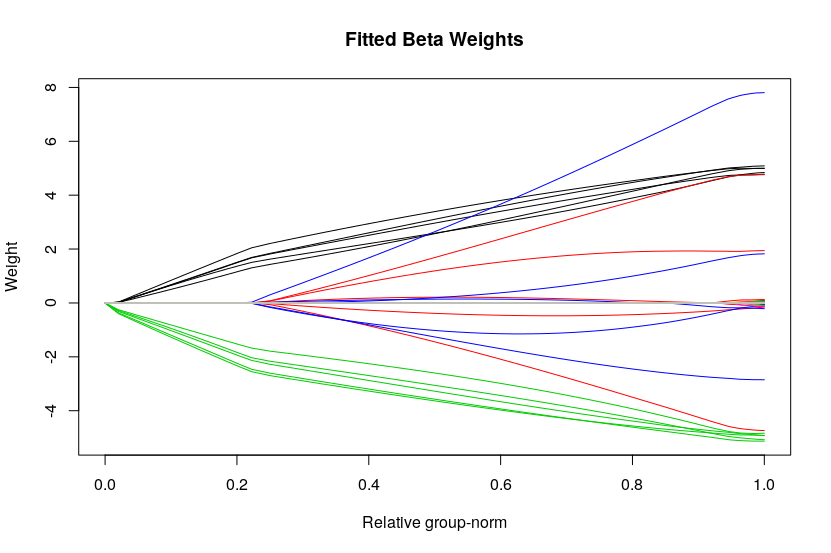
\includegraphics[scale=0.5]{fitted_beta_weights.png}

We can see that there are four active groups (all other groups remain 0 for all values on the x-axis): black, green, red and blue. By comparing this graph with the true beta in the code above, we can get a measure of how the algorithm is performing across the various lambda values.

The black group (which we see has 5 members) quickly becomes active as lambda is decreased, and eventually all values settle at a value of 5. This is evidently the first group, which was set to five 5's. Similarly, the green group becomes active and converges to five $-5$'s; this is third group. The other two groups are active but have predictors that are 0--we can see that the red group, for instance, has a 5, a 2, and a $-5$, and must be the second group.

From comparing this output graph with the true $\beta$, with which the data was generated, one might ask what the optimal $\lambda$, is, which recovers the true structure. In this case, it appears the small end of the lambda path results in the most accurate estimates.


\section{Comparison}

First we will compare the two algorithms within the sparsegl function, threestep and fourstep, for both accuracy and speed. Then, we compare our package with two other competing packages, the SGL package (which performs sparse group lasso, without predictor-discarding rules) and the gglasso package (which only performs group lasso, but uses predictor-discarding rules). Since the main contribution of this package is a fast algorithm for sparse group lasso, we pay particular attention to the speed difference between our algorithms and SGL.

For all comparisons, we use the R package microbenchmark, which compares two or more operations by performing them repeatedly (100 for our analysis) and collecting the times to perform each operation.

We can see that there is not a big difference in the time it takes to perform the threestep algorithm vs the fourstep algorithm. This is possibly a result of the simulated data used, and we believe that for some large datasets, the fourstep algorithm will outperform the threestep.

We also compare the actual output, in particular the beta matrix, to confirm that they are arriving at the same answers. For this comparison, the lambda path is about the same, but for the other packages (gglasso, SGL), the lambda path will in general be different, so some care must be taken in comparing the beta matrices.



\end{document}